\section{Referencia de la Clase Presupuesto\-View}
\label{classPresupuestoView}\index{PresupuestoView@{PresupuestoView}}
Muestra y administra la ventana con la informaci\'{o}n de un presupuesto.  


{\tt \#include $<$presupuestoview.h$>$}

Diagrama de herencias de Presupuesto\-View\begin{figure}[H]
\begin{center}
\leavevmode
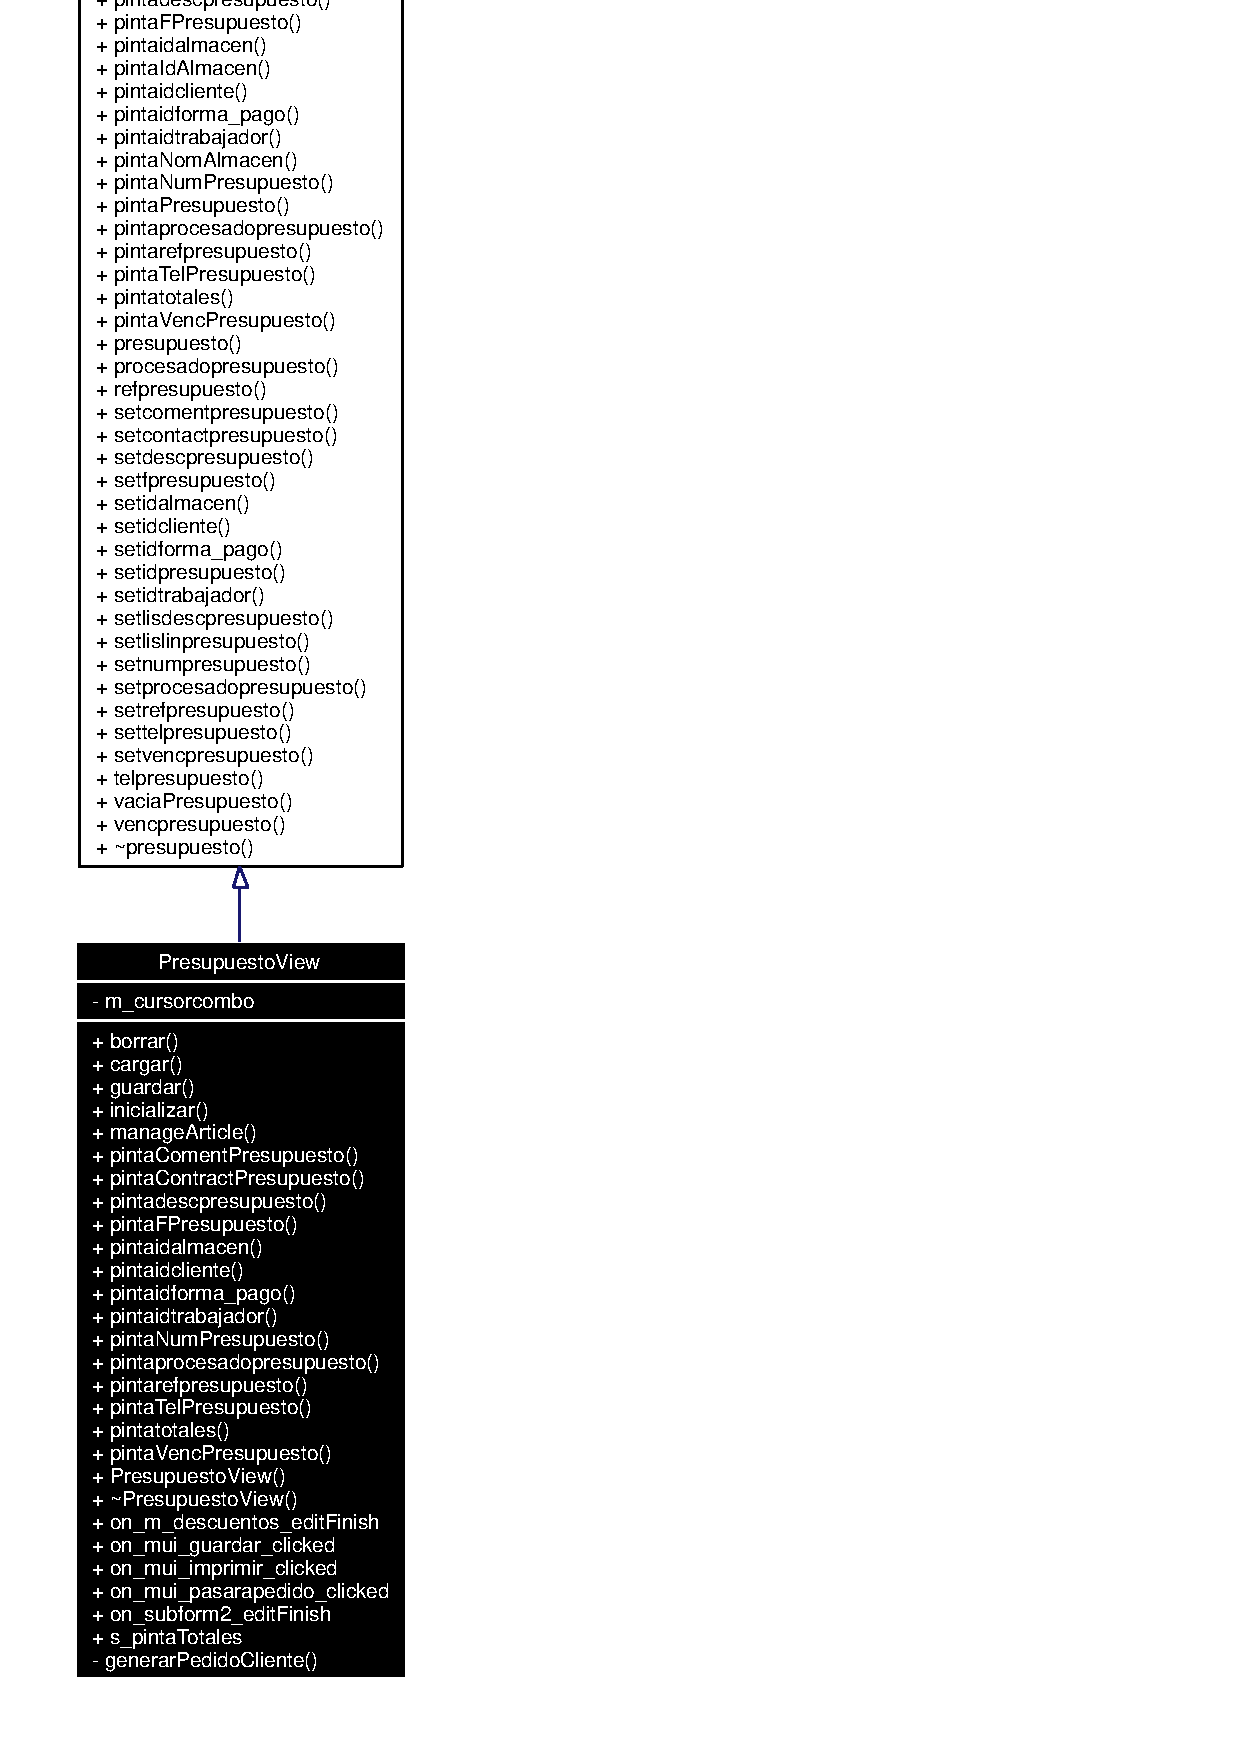
\includegraphics[width=97pt]{classPresupuestoView__inherit__graph}
\end{center}
\end{figure}
Diagrama de colaboraci\'{o}n para Presupuesto\-View:\begin{figure}[H]
\begin{center}
\leavevmode
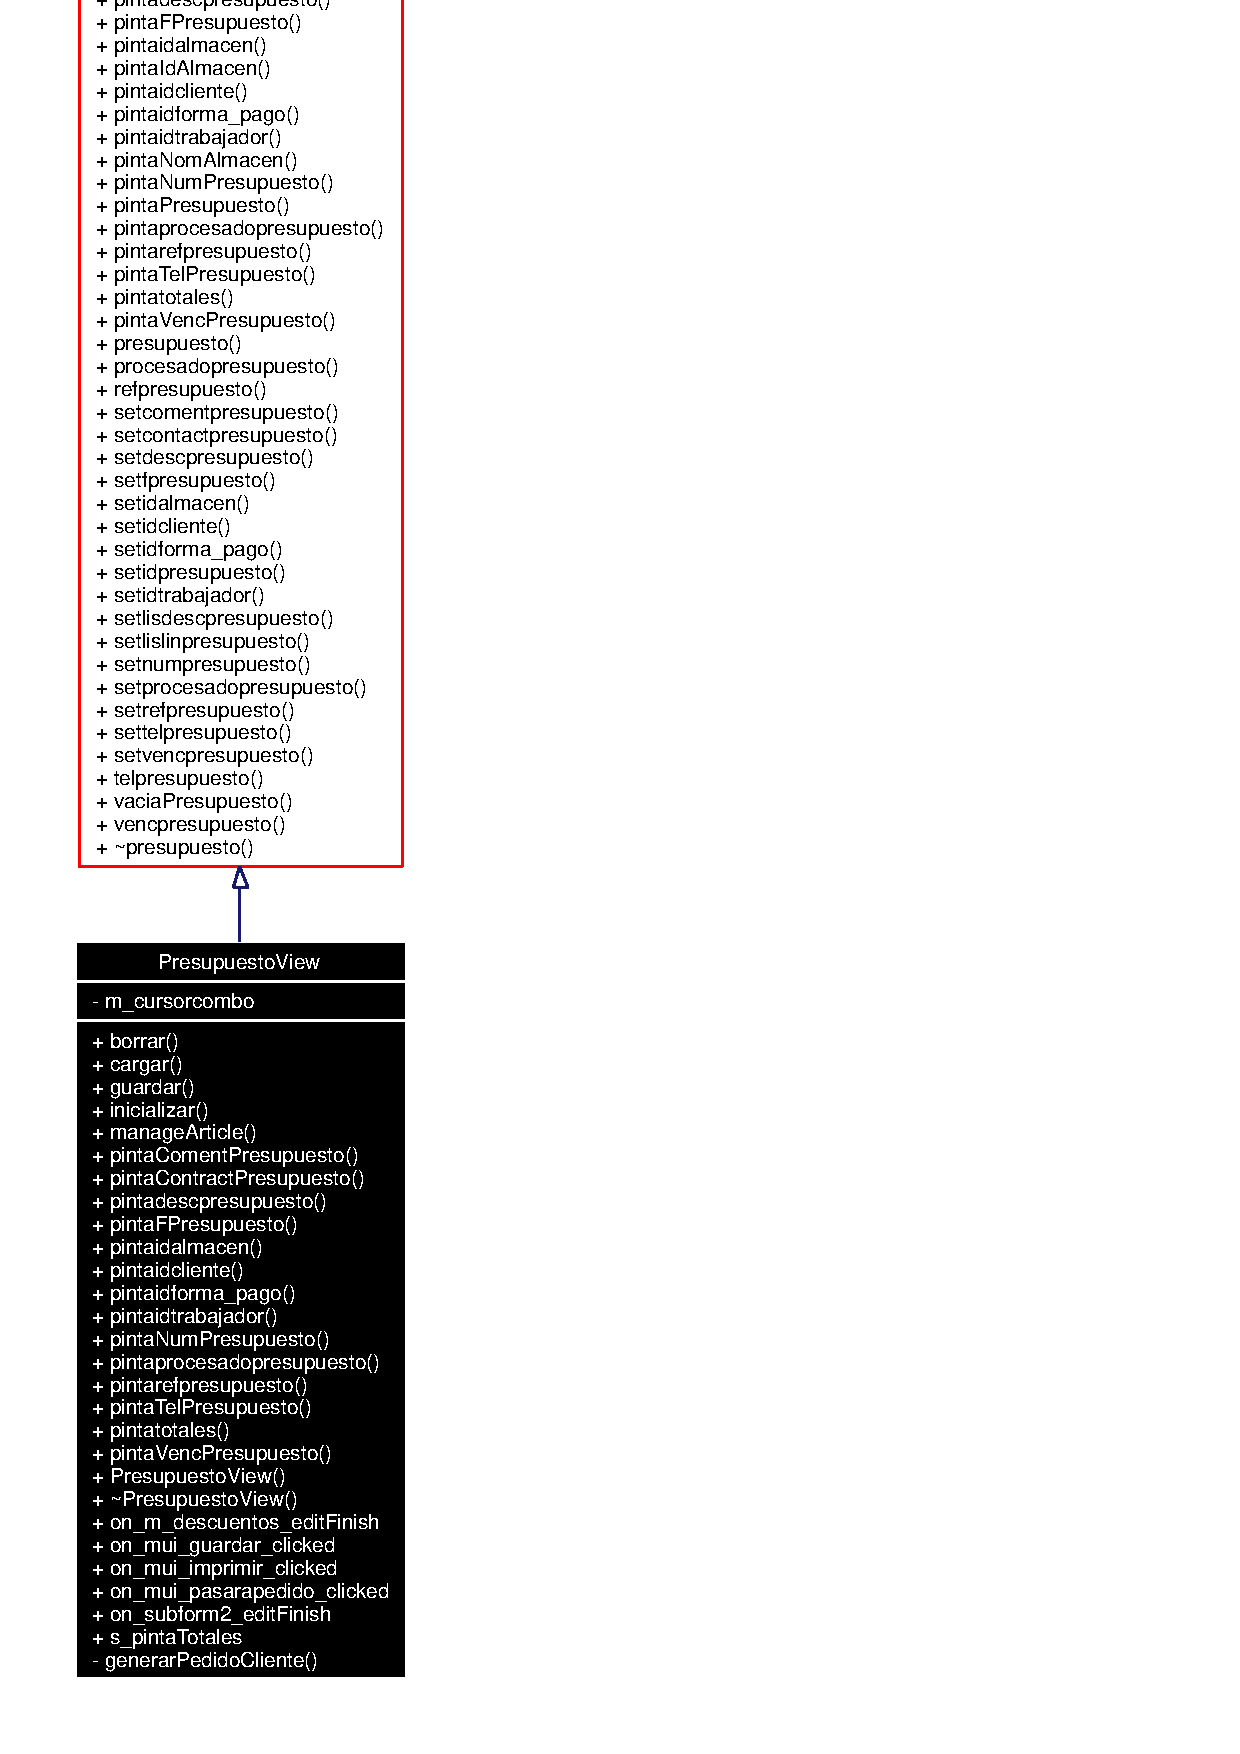
\includegraphics[width=97pt]{classPresupuestoView__coll__graph}
\end{center}
\end{figure}
\subsection*{Slots p\'{u}blicos}
\begin{CompactItemize}
\item 
virtual void {\bf on\_\-m\_\-descuentos\_\-edit\-Finish} (int, int)\label{classPresupuestoView_i0}

\item 
virtual void {\bf on\_\-mui\_\-guardar\_\-clicked} ()\label{classPresupuestoView_i1}

\item 
virtual void {\bf on\_\-mui\_\-imprimir\_\-clicked} ()\label{classPresupuestoView_i2}

\item 
virtual void {\bf on\_\-mui\_\-pasarapedido\_\-clicked} ()\label{classPresupuestoView_i3}

\item 
virtual void {\bf on\_\-subform2\_\-edit\-Finish} (int, int)\label{classPresupuestoView_i4}

\item 
virtual void {\bf s\_\-pinta\-Totales} ()\label{classPresupuestoView_i5}

\begin{CompactList}\small\item\em Este slot se activa cuando hay cambios en los subformularios. \item\end{CompactList}\end{CompactItemize}
\subsection*{M\'{e}todos p\'{u}blicos}
\begin{CompactItemize}
\item 
virtual int {\bf borrar} ()\label{classPresupuestoView_a0}

\item 
virtual int {\bf cargar} (QString id)
\begin{CompactList}\small\item\em Esta funcion carga un presupuesto. \item\end{CompactList}\item 
virtual int {\bf guardar} ()
\begin{CompactList}\small\item\em Estos metodos deben existir para poder trabajar con la clase Ficha. \item\end{CompactList}\item 
void {\bf inicializar} ()\label{classPresupuestoView_a3}

\begin{CompactList}\small\item\em Este metodo es llamado cuando hacemos un nuevo registro, pero no hay carga desde la base de datos. \item\end{CompactList}\item 
void {\bf manage\-Article} (int)\label{classPresupuestoView_a4}

\item 
void {\bf pinta\-Coment\-Presupuesto} (QString id)\label{classPresupuestoView_a5}

\item 
void {\bf pinta\-Contract\-Presupuesto} (QString id)\label{classPresupuestoView_a6}

\item 
void {\bf pintadescpresupuesto} (QString id)\label{classPresupuestoView_a7}

\item 
void {\bf pinta\-FPresupuesto} (QString id)\label{classPresupuestoView_a8}

\item 
void {\bf pintaidalmacen} (QString id)\label{classPresupuestoView_a9}

\item 
void {\bf pintaidcliente} (QString id)\label{classPresupuestoView_a10}

\item 
void {\bf pintaidforma\_\-pago} (QString id)\label{classPresupuestoView_a11}

\item 
void {\bf pintaidtrabajador} (QString id)\label{classPresupuestoView_a12}

\item 
void {\bf pinta\-Num\-Presupuesto} (QString id)\label{classPresupuestoView_a13}

\item 
void {\bf pintaprocesadopresupuesto} (QString id)\label{classPresupuestoView_a14}

\item 
void {\bf pintarefpresupuesto} (QString id)\label{classPresupuestoView_a15}

\item 
void {\bf pinta\-Tel\-Presupuesto} (QString id)\label{classPresupuestoView_a16}

\item 
void {\bf pintatotales} (Fixed iva, Fixed base, Fixed total, Fixed desc)\label{classPresupuestoView_a17}

\item 
void {\bf pinta\-Venc\-Presupuesto} (QString id)\label{classPresupuestoView_a18}

\item 
{\bf Presupuesto\-View} ({\bf company} $\ast$, QWidget $\ast$)
\end{CompactItemize}


\subsection{Descripci\'{o}n detallada}
Muestra y administra la ventana con la informaci\'{o}n de un presupuesto. 



\subsection{Documentaci\'{o}n del constructor y destructor}
\index{PresupuestoView@{Presupuesto\-View}!PresupuestoView@{PresupuestoView}}
\index{PresupuestoView@{PresupuestoView}!PresupuestoView@{Presupuesto\-View}}
\subsubsection{\setlength{\rightskip}{0pt plus 5cm}Presupuesto\-View::Presupuesto\-View ({\bf company} $\ast$ {\em comp}, QWidget $\ast$ {\em parent})}\label{classPresupuestoView_a19}


Disparamos los plugins con presupuesto\_\-imprimir\-Presupuesto.

Usurpamos la identidad de mlist y ponemos nuestro propio widget con sus cosillas.

Inicializamos la forma de pago para que no se quede sin ser pintada.

Disparamos los plugins por flanco descendente. 

\subsection{Documentaci\'{o}n de las funciones miembro}
\index{PresupuestoView@{Presupuesto\-View}!cargar@{cargar}}
\index{cargar@{cargar}!PresupuestoView@{Presupuesto\-View}}
\subsubsection{\setlength{\rightskip}{0pt plus 5cm}int Presupuesto\-View::cargar (QString {\em id})\hspace{0.3cm}{\tt  [virtual]}}\label{classPresupuestoView_a1}


Esta funcion carga un presupuesto. 

Tratamiento de excepciones. 

Reimplementado de {\bf presupuesto} {\rm (p.\,\pageref{classpresupuesto_a5})}.\index{PresupuestoView@{Presupuesto\-View}!guardar@{guardar}}
\index{guardar@{guardar}!PresupuestoView@{Presupuesto\-View}}
\subsubsection{\setlength{\rightskip}{0pt plus 5cm}int Presupuesto\-View::guardar ()\hspace{0.3cm}{\tt  [virtual]}}\label{classPresupuestoView_a2}


Estos metodos deben existir para poder trabajar con la clase Ficha. 

Disparamos los plugins con presupuesto\_\-imprimir\-Presupuesto. 

Reimplementado de {\bf presupuesto} {\rm (p.\,\pageref{classpresupuesto})}.

La documentaci\'{o}n para esta clase fu\'{e} generada a partir de los siguientes archivos:\begin{CompactItemize}
\item 
presupuestoview.h\item 
presupuestoview.cpp\end{CompactItemize}
